\section{Results} % Approx word count = 1000 words (total = 2750)

\begin{figure*}
    \centering
    \begin{subfigure}{\columnwidth}
        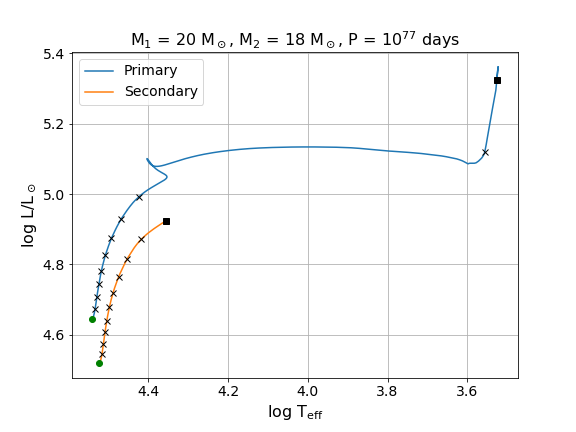
\includegraphics[width=\textwidth]{figures/results1/fig_HR_M20_Sin.png}
        \captionsetup{width=.9\columnwidth}
        \caption{HR diagram showing the evolution tracks for the M$_1$ = 20 M$_{\sun}$ system as non-interacting single stars.
        Note both tracks terminate simultaneously when the primary completes core helium burning.}
        \label{subfig:20Msol_HR_Sin}
    \end{subfigure}
    \hfill
    \begin{subfigure}{\columnwidth}
        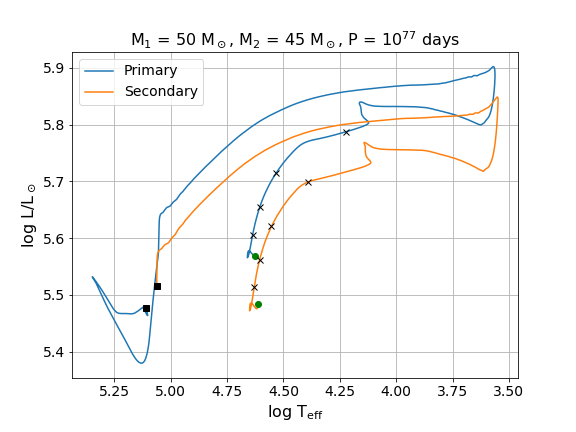
\includegraphics[width=\textwidth]{figures/results1/fig_HR_M50_Sin.png}
        \captionsetup{width=.9\columnwidth}
        \caption{As figure \ref{subfig:20Msol_HR_Sin} for the M$_1$ = 50 M$_{\sun}$ system. \newline \newline}
        \label{subfig:50Msol_HR_Sin}
    \end{subfigure}
    
    \begin{subfigure}{\columnwidth}
        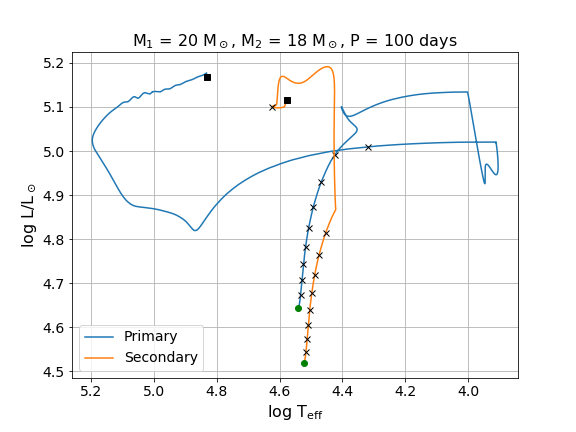
\includegraphics[width=\columnwidth]{figures/results1/fig_HR_M20_P100.png}
        \captionsetup{width=.9\columnwidth}
        \caption{HR diagram showing the evolution tracks for the M$_1$ = 20 M$_{\sun}$ interacting binary system at initial period P = 100 days.}
        \label{subfig:20Msol_HR_Bin}
    \end{subfigure}
    \hfill
    \begin{subfigure}{\columnwidth}
        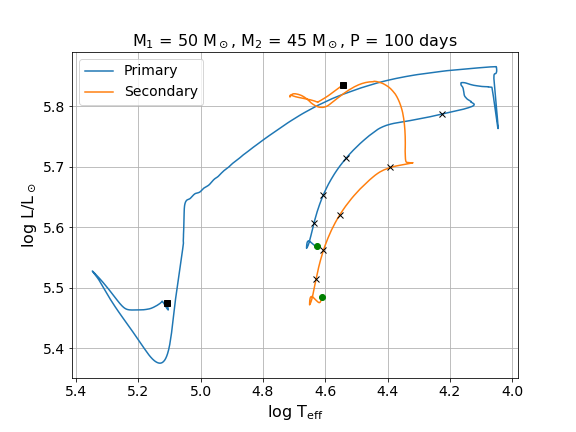
\includegraphics[width=\columnwidth]{figures/results1/fig_HR_M50_P100.png}
        \captionsetup{width=.9\columnwidth}
        \caption{As figure \ref{subfig:20Msol_HR_Bin} for the M$_1$ = 50 M$_{\sun}$ system. \newline}
        \label{subfig:50Msol_HR_Bin}
    \end{subfigure}
    
    \begin{subfigure}{\columnwidth}
        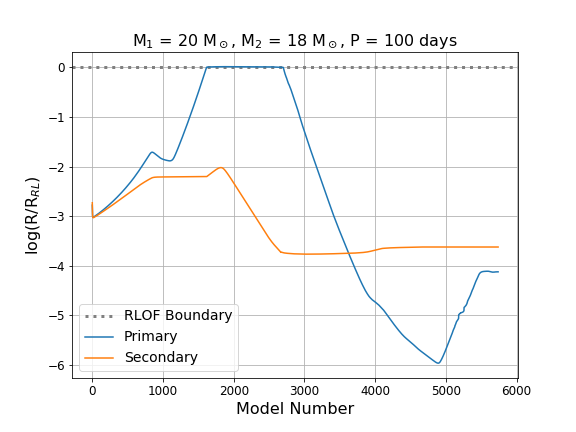
\includegraphics[width=\columnwidth]{figures/results1/fig_RLOF_M20_P100.png}
        \captionsetup{width=.9\columnwidth}
        \caption{Stellar radius as a fraction of Roche lobe radius for the M$_1$ = 20 M$_{\sun}$ system. Roche lobe overflow occurs while $\log$(R/R\textsubscript{RL}) = 0.}
        \label{subfig:20Msol_RLOF}
    \end{subfigure}
    \hfill
    \begin{subfigure}{\columnwidth}
        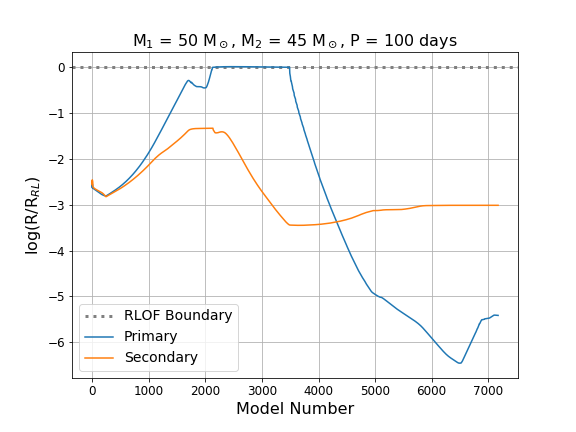
\includegraphics[width=\columnwidth]{figures/results1/fig_RLOF_M50_P100.png}
        \captionsetup{width=.9\columnwidth}
        \caption{As figure \ref{subfig:20Msol_RLOF} for the M$_1$ = 50 M$_{\sun}$ system. \newline}
        \label{subfig:50Msol_RLOF}
    \end{subfigure}
\caption{Diagrams comparing the evolution of M$_1$ = 20 M$_{\sun}$ (left) and M$_1$ = 50 M$_{\sun}$ (right) binary systems with their single star counterparts. The HR evolution tracks begin at the green circle as zero-age main sequence stars, each $\times$ marks 10$^6$ years of evolution. Note that the stellar radius plots are shown in terms of the simulation model number (i.e. non-linear timesteps) to give a qualitative impression of the RLOF process (which happens on a very short timescale relative to the age of the star).}
\label{fig:SinglevsBinary}
\end{figure*}

\begin{figure*}
    \centering
    \begin{subfigure}{\columnwidth}
        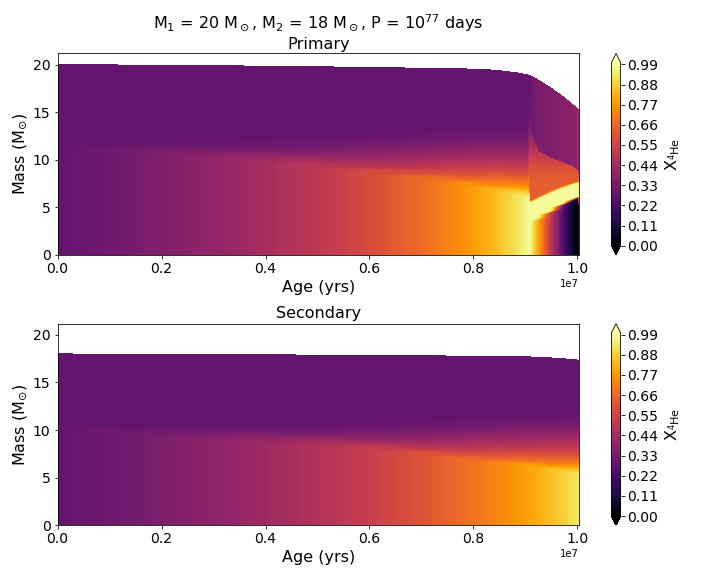
\includegraphics[width=\textwidth]{figures/results1/fig_He4_Age_M20_Sin.png}
        \captionsetup{width=.9\columnwidth}
        \caption{He-4 composition for the single star simulation.}
        \label{subfig:20Msol_He4_Sin}
    \end{subfigure}
    \begin{subfigure}{\columnwidth}
        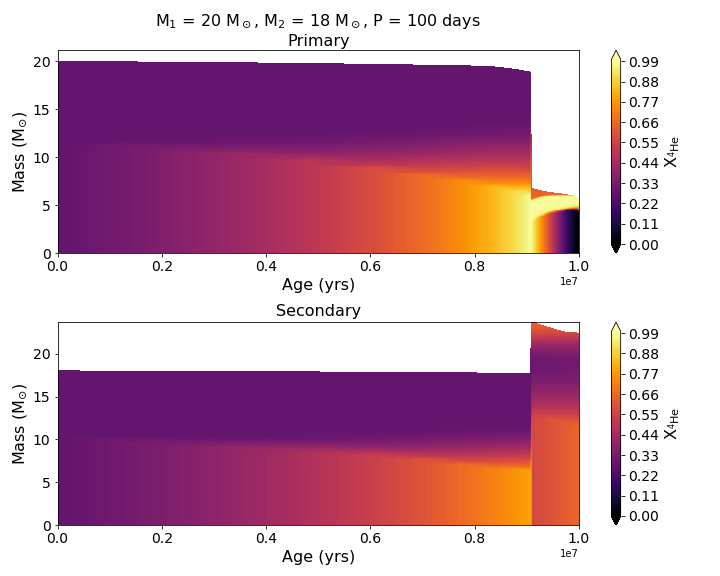
\includegraphics[width=\textwidth]{figures/results1/fig_He4_Age_M20_P100.png}
        \captionsetup{width=.9\columnwidth}
        \caption{He-4 composition for the P = 100 days binary simulation.}
        \label{subfig:20Msol_He4_Bin}
    \end{subfigure}
    \begin{subfigure}{\columnwidth}
        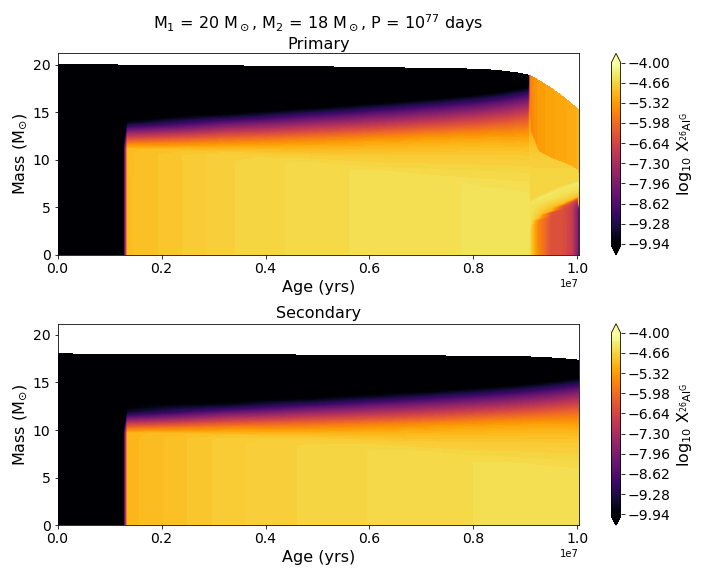
\includegraphics[width=\textwidth]{figures/results1/fig_Al26_Age_M20_Sin.png}
        \captionsetup{width=.9\columnwidth}
        \caption{$^{26}$Al composition for the single star simulation.}
        \label{subfig:20Msol_Al26_Sin}
    \end{subfigure}
    \begin{subfigure}{\columnwidth}
        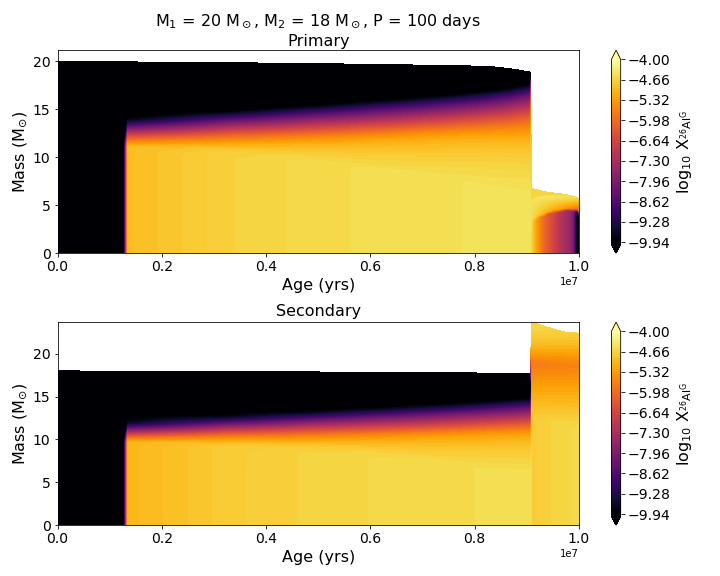
\includegraphics[width=\textwidth]{figures/results1/fig_Al26_Age_M20_P100.png}
        \captionsetup{width=.9\columnwidth}
        \caption{$^{26}$Al composition for the P = 100 days binary simulation.}
        \label{subfig:20Msol_Al26_Bin}
    \end{subfigure}
\caption{Figures showing the chemical evolution of the M$_1$ = 20 M$_{\sun}$ system as single stars (left) and binary stars with initial period 100 days (right).
The y-axis shows the mass of the star, while the colour gives the composition for material in the star at that mass coordinate(i.e. at the radius for which a sphere of that radius centred on the stellar core would contain a given mass).
Note that He-4 and $^{26}$Al are both created in hydrogen-burning stages and destroyed in helium-burning stages.
}
\label{fig:20Msol_Composition}
\end{figure*}

\begin{figure*}
    \begin{subfigure}{\columnwidth}
        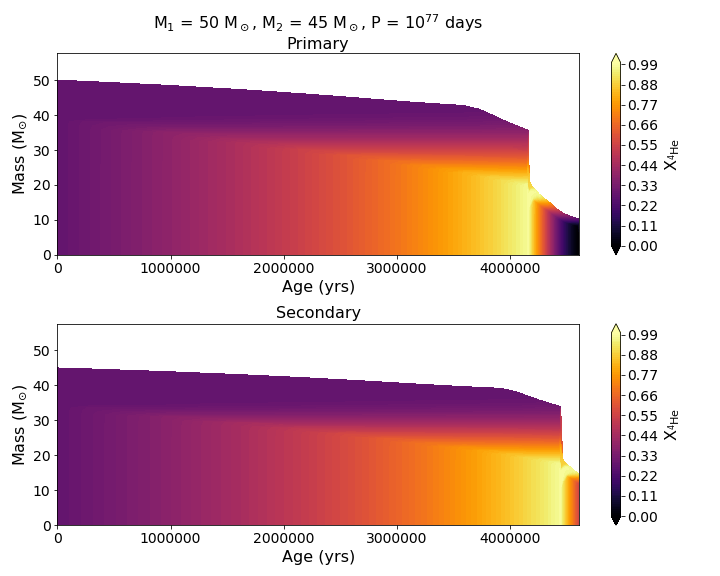
\includegraphics[width=\textwidth]{figures/results1/fig_He4_Age_M50_Sin.png}
        \captionsetup{width=.9\columnwidth}
        \caption{He-4 composition for the single star simulation.}
        \label{subfig:50Msol_He4_Sin}
    \end{subfigure}
    \begin{subfigure}{\columnwidth}
        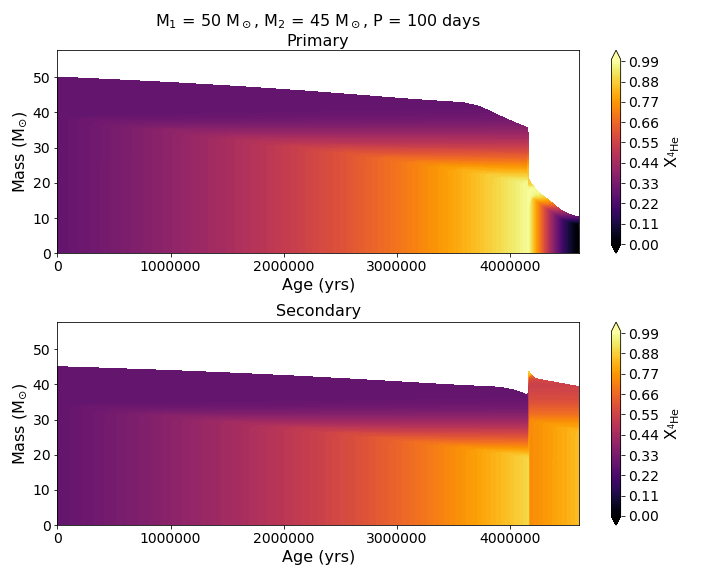
\includegraphics[width=\textwidth]{figures/results1/fig_He4_Age_M50_P100.png}
        \captionsetup{width=.9\columnwidth}
        \caption{He-4 composition for the P = 100 days binary simulation.}
        \label{subfig:50Msol_He4_Bin}
    \end{subfigure}
    \begin{subfigure}{\columnwidth}
        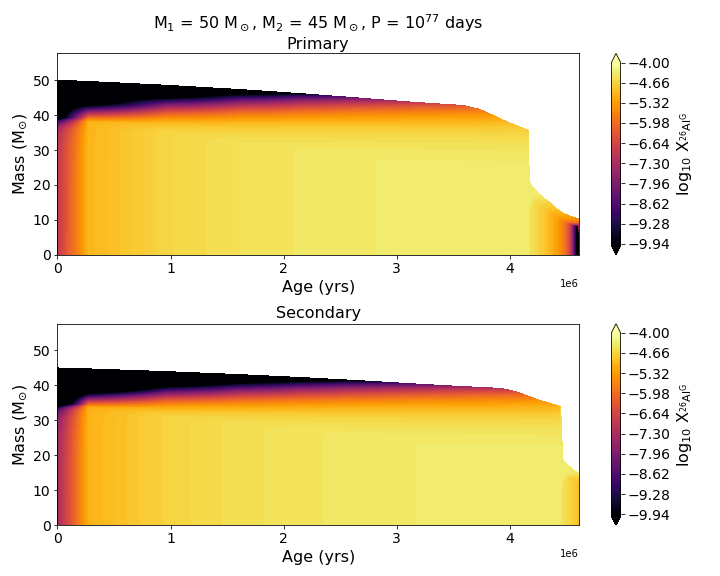
\includegraphics[width=\textwidth]{figures/results1/fig_Al26_Age_M50_Sin.png}
        \captionsetup{width=.9\columnwidth}
        \caption{$^{26}$Al composition for the single star simulation.}
        \label{subfig:50Msol_Al26_Sin}
    \end{subfigure}
    \begin{subfigure}{\columnwidth}
        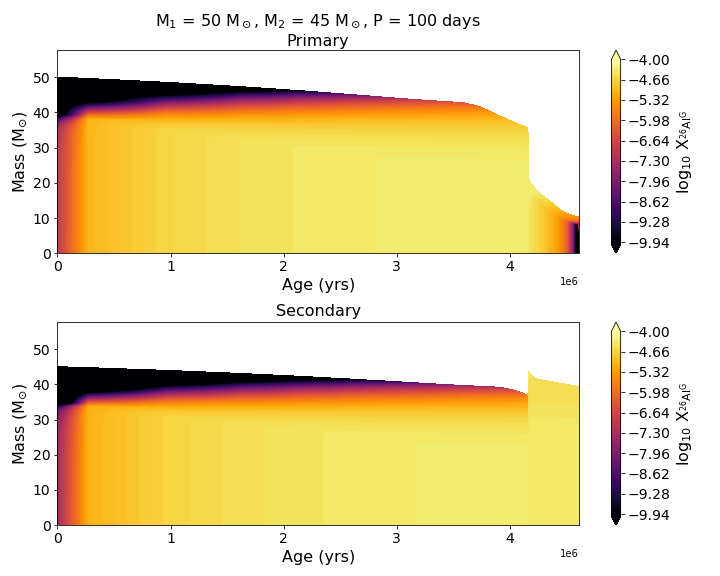
\includegraphics[width=\textwidth]{figures/results1/fig_Al26_Age_M50_P100.png}
        \captionsetup{width=.9\columnwidth}
        \caption{$^{26}$Al composition for the P = 100 days binary simulation.}
        \label{subfig:50Msol_Al26_Bin}
    \end{subfigure}
\caption{As figure \ref{fig:20Msol_Composition} for the M$_1$ = 50 M$_{\sun}$ system.}
\label{fig:50Msol_Composition}
\end{figure*}

The effects of binary interaction on $^{26}$Al yield was found to differ significantly between each primary mass: increasing for the 20 M$_{\sun}$ system, but decreasing for the 50 M$_{\sun}$ system.
The following sections examine each result in turn.

\subsection{20 M$_{\sun}$} \label{20Msol}

\subsubsection{Single Star Evolution}

% Evolution
Figure \ref{subfig:20Msol_HR_Sin} shows the evolution of both the 20 M$_{\sun}$ primary and 18 M$_{\sun}$ secondary as non-interacting single stars.
Initially, both stars move across the main sequence, producing $^{26}$Al in the core (see figure \ref{subfig:20Msol_Al26_Sin}).
The primary star exhausts core hydrogen at $\sim$8.5 Myr (see figure \ref{subfig:20Msol_He4_Sin}) and enters the next stage of its evolution, cooling and expanding at roughly constant luminosity.
Luminosity then increases coinciding with the ignition of helium at $\sim$9.2 Myr.
During this stage, $^{26}$Al is destroyed in the core. Mixing within the stellar envelope also brings some to the surface, where it is ejected by stellar winds (see figure \ref{subfig:20Msol_Al26_Sin}).
The simulation terminates once the primary completes core helium burning at $\sim$10 Myr (see figure \ref{subfig:20Msol_He4_Sin}).

% Yields
The primary loses 4.82 M$_{\sun}$ during single star evolution, ejecting $2.35\times10^{-5}$ M$_{\sun}$ of $^{26}$Al. Note that this is an underestimate because there is still some surface $^{26}$Al remaining at end of the simulation.
However, since the remaining lifetime of the star is at most a few thousand years \citep{Iliadis2015}, there will be minimal additional $^{26}$Al yields before the supernova.

\subsubsection{Binary Star Evolution}

Figure \ref{subfig:20Msol_HR_Bin} shows the evolution of the same stars in a close binary system with an initial period of 100 days.
The stars evolve as above until $\sim$8.5 Myr when the primary exhausts core hydrogen, expands, and fills its Roche lobe (see figure \ref{subfig:20Msol_RLOF}).
Material is exchanged in a single instance of case B mass transfer, which dramatically alters the evolution tracks of both stars.
Figures \ref{subfig:20Msol_He4_Sin} and \ref{subfig:20Msol_He4_Bin} show that the primary's core is largely unaltered while almost the entire envelope is stripped from the star.
The secondary, meanwhile, is rejuvenated by mixing in some of the hydrogen from the accreted material, thus extending its main-sequence lifespan (see \cite{2007MNRAS.376...61D} for more details on this phenomenon).

% Primary yields.
About 12 M$_{\sun}$ of material with a mean $^{26}$Al abundance between $\sim$10$^{-5}$ to $\sim$10$^{-4}$ is lost from the primary, half of which is accreted onto the secondary. The other half is ejected, giving a primary yield of $9.04\times10^{-5}$ M$_{\sun}$ (nearly 4$\times$ the single star yield).
% Secondary yields.
The secondary yields are also increased due to ejection of accreted $^{26}$Al from the surface (see table \ref{tab:data1}).
However, there is little value in comparing these yields at this stage since the secondary evolution was cut short. Continued secondary evolution is discussed in more detail below (see section \ref{Secondaries}).

\subsection{50 M$_{\sun}$}

\subsubsection{Single Star Evolution}

% Evolution
Figure \ref{subfig:50Msol_HR_Sin} shows the evolution of both the 50 M$_{\sun}$ primary and 45 M$_{\sun}$ secondary as non-interacting single stars.
Compared to the $\sim$20 M$_{\sun}$ stars, these stars evolve much faster, lasting only 4.61 Myr before exhausting core helium in the primary.
Note that as a result, both stars complete hydrogen-burning during the same simulation, although the secondary does not complete helium-burning.
Over the course of main sequence evolution, $^{26}$Al is produced in the convective cores which quickly reaches a composition approaching $\sim$10$^{-4}$ in the first Myr.
By $\sim$3.5 Myr for the primary and $\sim$4.0 Myr for the secondary, stellar winds have completely ejected the upper envelope (see figure \ref{subfig:50Msol_Al26_Sin}) and begin ejecting $^{26}$Al. About 10 M$_{\sun}$ is lost from the primary overall during this stage.
Once helium-burning begins in the primary at $\sim$4.2 Myr (see figure \ref{subfig:50Msol_He4_Sin}), stellar winds become much stronger and the star ejects both its entire envelope and the hydrogen shell, leaving the hot, helium-burning core behind as a WR star \citep[see][]{Carroll2007}.
A further $\sim$30 M$_{\sun}$ of material is lost from the primary during this stage.

% Yields
The primary loses 39.68 M$_{\sun}$ during single star evolution, ejecting $9.23\times10^{-4}$ M$_{\sun}$ of $^{26}$Al.
The secondary loses 30.26 M$_{\sun}$ over the same period, ejecting $6.96\times10^{-4}$ M$_{\sun}$ of $^{26}$Al.
The combined $^{26}$Al yield is $1.62\times10^{-3}$ M$_{\sun}$. Since both stars became WR stars, continued evolution is unlikely to yield much more $^{26}$Al before the supernova for either star.

\subsubsection{Binary Star Evolution}

Figure \ref{subfig:50Msol_HR_Bin} shows the evolution of the same stars in a close binary system with an initial period of 100 days.
Mass transfer occurs at $\sim$4.2 Myr when the primary exhausts core hydrogen, expands, and fills its Roche lobe (see figure \ref{subfig:50Msol_RLOF}).
Since stars of this mass become WR, the mass loss profile of the primary is almost identical to its single star evolution (compare figures \ref{subfig:50Msol_He4_Sin} \& \ref{subfig:50Msol_He4_Bin}). Note, however, that some of this lost mass is accreted onto the secondary and does not contribute to yields. Thus, the primary yield is reduced to by about a third to $6.53\times10^{-04}$.

As in the 18 M$_{\sun}$ case, the 45 M$_{\sun}$ secondary's core is rejuvenated by accreted hydrogen \citep[see][]{2007MNRAS.376...61D}. The resulting extension of its main sequence lifespan goes beyond the length of the simulation.
This leads to dramatically reduced secondary yields during the simulated period (see table \ref{tab:data1}), however this is misleading since continued secondary evolution through the WR stage would eject the accreted $^{26}$Al leading to a total yield comparable to the combined single star yield ($\sim$10$^{-3}$ M$_{\sun}$).
However, this would not be the case for systems with a WR primary and a lower mass secondary star that does not become WR even after accreting material.

\subsection{Varying Orbital Period} \label{Period}

\begin{figure}
    \centering
    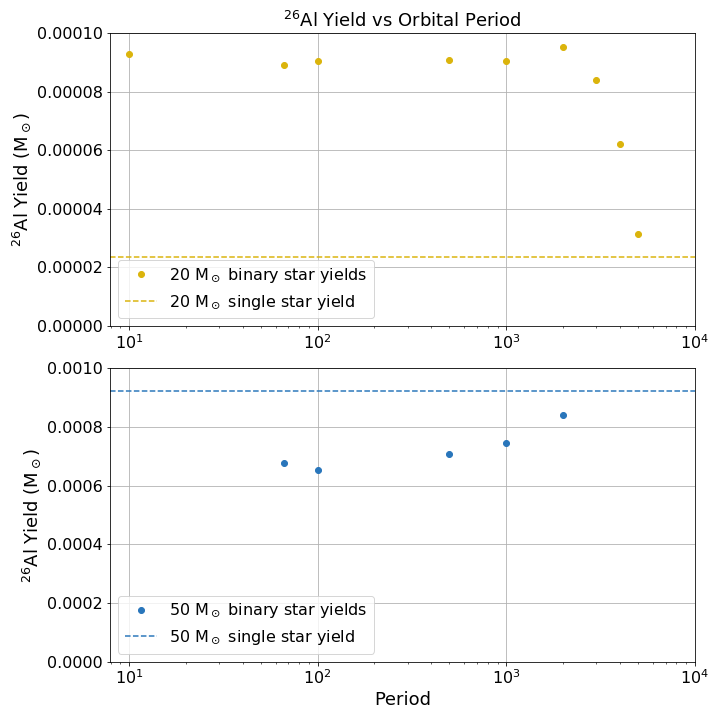
\includegraphics[width=\columnwidth]{figures/results1/fig_YieldvsPeriod.png}
    \captionsetup{width=\columnwidth}
    \caption{$^{26}$Al yield from binary systems of primary masses 20 M$_{\sun}$ and 50 M$_{\sun}$ against orbital period.}
    \label{fig:Period}
\end{figure}

While the basic result of the binary interaction changes depending on the mass of the star in question, the details of the mass transfer depend on the separation between the stars, or equivalently, their orbital period\footnote{Period $P$ and separation $a$ are fundamentally linked by \textit{Kepler's Third Law}: $P^2 = \frac{4\pi}{GM}a^3$.}.
In particular, more distant stars (i.e. those with longer periods) have larger Roche lobes as estimated by the following equation from \cite{1983ApJ...268..368E}:
\begin{equation}
    \frac{R_{RL}}{a}=\frac{0.49q^{2/3}}{0.6q^{2/3}+\ln{1+q^{1/3}}}
\end{equation}
where $R_{RL}$ approximates the Roche lobe radius, $a$ is the separation between stars, and $q$ is the mass ratio $\frac{M_1}{M_2}$.
Thus, they will need to expand to a larger radius to initiate mass transfer than stars with a shorter period.

The effect of the initial period on $^{26}$Al yield was investigated for initial periods 10, 66.2\footnotemark, 100, 500, 1000, and 2000 days.
The key result is that mass transfer occurs sooner in the evolution of each star for systems with a shorter initial period, as can be seen in figure \ref{fig:Period_HR}.
\footnotetext{P = 66.2 days was chosen to allow a direct comparison with a similar simulation by \cite{2019ApJ...884...38B}.}
Further 20 M$_{\sun}$ simulations were run for 3000, 4000, and 5000 day periods to generate more data for cases with particularly late interaction.
The results can be seen in figure \ref{fig:Period}\footnote{Note that the P = 10 days, M$_1$ = 50 M$_{\sun}$ yield was not included. This is because the system evolved into a contact binary, and thus invalidated the assumption of spherical symmetry used by the code.} and table \ref{tab:data1}.
$^{26}$Al yields were found generally constant with respect to period for case B mass transfer at both masses. Case B was also found to be the most commonly occurring type of mass transfer for a flat distribution of initial periods.

The 20 M$_{\sun}$ primary ejected $\sim$9$\times$10$^{-5}$ M$_{\sun}$ of $^{26}$Al after total mass loss of $\sim$14 M$_{\sun}$ for P $\leq$ 1000 days, compared with 2.35$\times$10$^{-5}$ M$_{\sun}$ from a loss of $\sim$5 M$_{\sun}$ for single star evolution.
At higher periods, less mass was lost as the primary evolved out of RLOF before the mass transfer could complete, leading to yields that approach the single star values as period is increased.

The 50 M$_{\sun}$ stars always lost $\sim$40 M$_{\sun}$ regardless of period.
The primary yields were reduced from 9.23$\times$10$^{-4}$ M$_{\sun}$ to $\sim$6$\times$10$^{-4}$ M$_{\sun}$ for P $\leq$ 1000 days due to accretion onto the secondary.
At higher periods, the secondary accreted less mass and experienced less hydrogen rejuvenation. In the P = 2000 days case, the effect was so minor that the secondary began helium-burning within the simulation and the resulting mass loss led to a combined yield of 1.61$\times$10$^{-3}$ M$_{\sun}$, in-line with the combined single star yield (see table \ref{tab:data1}).

\subsection{Varying Mass Transfer Efficiency}

\begin{figure}
    \centering
    \begin{subfigure}{\columnwidth}
        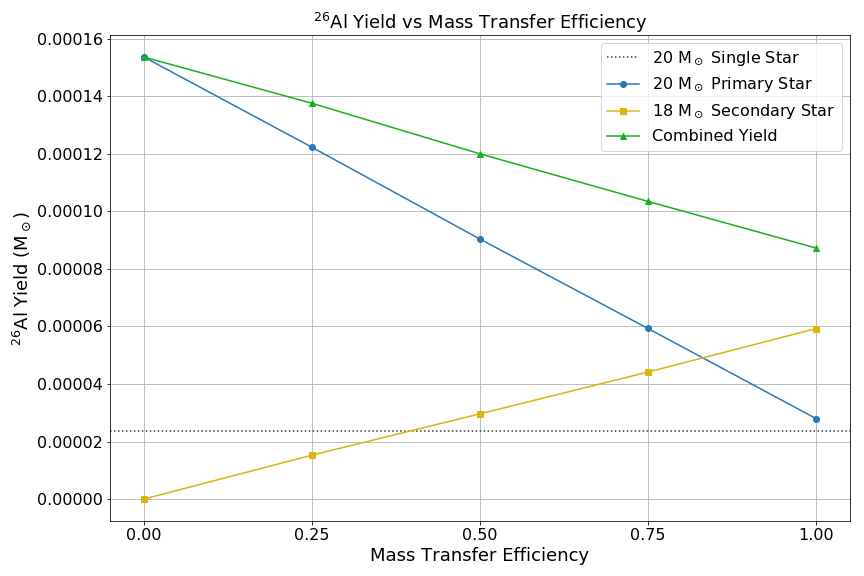
\includegraphics[width=\columnwidth]{figures/results2/fig_YieldvsMTE.png}
        \caption{Primary and secondary $^{26}$Al yields from system evolution up to the end of core helium-burning in the primary star. For comparison, the dotted line shows the yield for the primary evolved as a single star.}
        \label{subfig:MTE1}
    \end{subfigure}
    \begin{subfigure}{\columnwidth}
        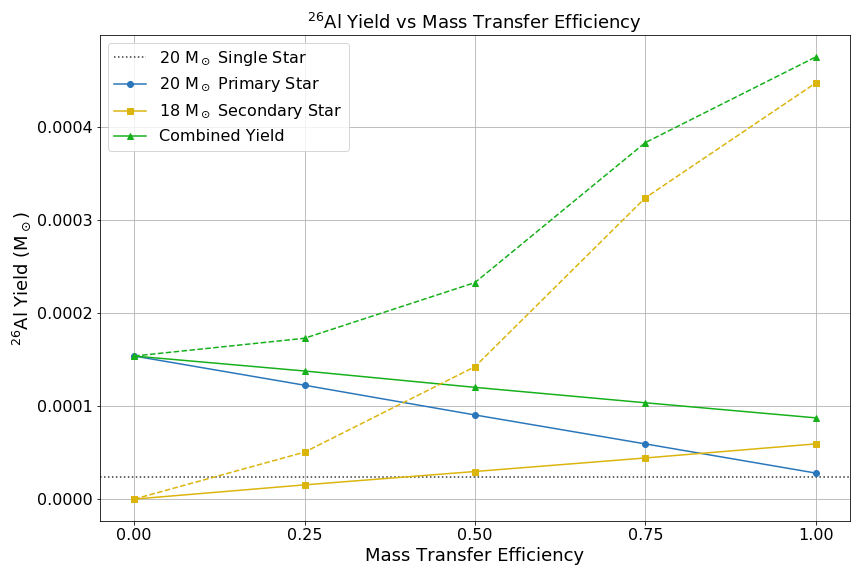
\includegraphics[width=\columnwidth]{figures/results2/fig_YieldvsMTE_2.png}
        \caption{As figure \ref{subfig:MTE1}, with dashed lines showing the binary yields plus additional yields from continued evolution of the secondary star as a single star (i.e. assuming no further binary interaction occurs).}
        \label{subfig:MTE2}
    \end{subfigure}
    \captionsetup{width=\columnwidth}
    \caption{The effect of mass transfer efficiency $\beta$ on $^{26}$Al yield for binary systems with M$_1$ = 20 M$_{\sun}$, M$_2$ = 18 M$_{\sun}$ and an initial period P = 100 days.}
    \label{fig:MTE}
\end{figure}

The effect of mass transfer efficiency $\beta$ on $^{26}$Al yield was investigated using values of $\beta$: 0.00, 0.25, 0.50, 0.75, and 1.00.
Given the minimal effect of binary interactions on the 50 M$_{\sun}$ system (see above), these simulations focused only on the 20 M$_{\sun}$ system at a period of 100 days (this corresponds to case B mass transfer, found above to be the most common -- see section \ref{Period}.).

The results can be seen in figure \ref{subfig:MTE1} and table \ref{tab:data2}.
There are two key points:
\begin{enumerate}
    \item Yields are increased (compared to single star yields) regardless of $\beta$ due to increased surface $^{26}$Al abundance on both stars after RLOF.
    \item The mass lost from the primary is the same in each case ($\sim$12 M$_{\sun}$ from RLOF). Since RLOF yield is proportional to both mass lost and $\beta$ there is a linear decrease in primary yields with increased $\beta$. Conversely, there is a linear increase in secondary yields due to wind mass loss rates increasing with angular momentum as mass is accreted (see section \ref{Method2}).
\end{enumerate}

While the combined yields were found to decrease with $\beta$ (from 1.54$\times$10$^{-4}$ at $\beta$ = 0 to 8.93$\times$10$^{-5}$ at $\beta$ = 1) the increased mass loss rates after accretion indicate the potential for increased yields from the secondaries, if allowed to complete their evolution.

\subsubsection{Continuing the Secondary Evolution} \label{Secondaries}
Once the primary stars complete core helium burning, the remaining $^{26}$Al yields are limited (see section \ref{20Msol}).
However, the less-evolved secondary stars still retain a significant $^{26}$Al composition at this time, especially in cases with high $\beta$.
To investigate these potential $^{26}$Al yields, the secondary star evolution was completed in single star mode.

The results can be seen in figure \ref{subfig:MTE2} and table \ref{tab:data2}, and indicate that the secondary stars could dramatically increase the system $^{26}$Al yield, if left to evolve without further binary interaction.
%After mass transfer, the secondaries' evolution paths were found to be roughly similar to those of single stars of masses equal to the new masses (see figures \ref{fig:MTE_HR}).
For 0 < $\beta$ $\leq$ 0.50, this led to evolution tracks a little higher in luminosity and evolution speed than the $\beta$ = 0 track, with stronger winds, greater mass loss, and correspondingly higher yields.
For $\beta$ $\geq$ 0.75, the secondary stars reached sufficient masses to become WR stars: ejecting nearly all of the $^{26}$Al produced by both stars.
At $\beta$ = 1, the secondary star ejected 18.2 M$_{\sun}$ of material during the continued evolution (more than its initial mass), resulting in a combined system $^{26}$Al yield of 4.75$\times$10$^{-4}$ (> 3 times the $\beta=0$ yield).